\documentclass[11pt,oneside]{book}
%Use the XJTLU Latex style
\usepackage{xjtlu}
%***********************************************
%Modify the following 5 items
%***********************************************
%The title of your report
\reporttitle{How to use the XJTLU \LaTeX{ }template to \\ write your academic article (Beta)}
%Your name
\student{Fei Cheng}
%Your module
\module{EEE \LaTeX{ }Tutorial}
%Your teacher
\lecturer{Mr.Cheng}
%The date
\finishdate{April/6/2013}

\begin{document}
% set line spacing to 1.5B
\baselineskip = 17pt
%Insert a cover with XJTLU logo into the first page
\thispagestyle{empty}
\newcommand\nbvspace[1][3]{\vspace*{\stretch{#1}}}
\newcommand\nbstretchyspace{\spaceskip0.5em plus 0.25em minus 0.25em}
\newcommand{\nbtitlestretch}{\spaceskip0.6em}
\newcommand{\psubtitle}[1]{\large\textit{{#1}}\\\normalsize}
\newcommand{\ptitle}[1]{\huge\textbf{{#1}}\\\normalsize}
\begin{center}
\begin{figure}
\centering

\includegraphics[width=10cm]{xjtlu.eps}
\label{fig:logo}
\end{figure}
\nbvspace[1]
%\psubtitle{Experimental Report}
\ptitle{\rtt}
\nbvspace[1]

\end{center}
\begin{flushleft}

\begin{table}[!hbp]
\centering
\begin{tabular}{p{2.5cm} p{5cm}}

   % after \\: \hline or \cline{col1-col2} \cline{col3-col4} ...
   \\
  \Large \textbf{Author:}&\Large\stu \\  \\
  \Large \textbf{Module:}&\Large \modu \\  \\
  \Large \textbf{Lecturer:}&\Large \lect \\   \\
   \Large\textbf{Date:}& \Large \dat \\
 \end{tabular}
\end{table}
\normalsize
\nbvspace[1]
\end{flushleft}

%Use Roman number
\frontmatter
%***********************************************
%Write Abstract in the following part
%***********************************************
\chapter{Abstract}

Write your abstract here.

\textbf{Key words:} key words.
%***********************************************
%Insert a contents automatically
%***********************************************
\tableofcontents
\addcontentsline{toc}{chapter}{Contents}

% List of figures  not put in table of contents by default so add it separately
%\listoffigures
%\addcontentsline{toc}{chapter}{List of Figures}

%\printglossary
%\addcontentsline{toc}{chapter}{Nomenclature}

\mainmatter

%***********************************************
%Begin your report!!
%***********************************************
%   Insert a chapter : \chapter{chapter name}\label{cpt:name}
%       Insert a section : \section{section name}\label{sec:name}
%           Insert a subsection : \subsection{subsection name}\label{subsec:name}
%   **Note: The label name is used for cross-referencing.
%       eg. \ref{cpt:name} can refer the number of this chapter.
\chapter{chapter 1}\label{cpt:c1}


\section{Section 1.1}\label{sec:s11}

How to add a citation or reference \cite{lun2000study}. Please open the file reference.bib to check how to 
add a citation. Google scholar and IEEE Xplore provide the right format of citation. You can copy Bibtex format
to reference.bib and use cite command in tex file to cite the reference.

In Section \ref{sec:s21}, it will introduce how to add a figure.


\chapter{chapter 2}\label{cpt:c2}

\section{Section 2.1}\label{sec:s21}

Two way can be used to add a figure.

Method 1: In Fig \ref{fig:example1}.

\begin{figure}[htp]
\centering
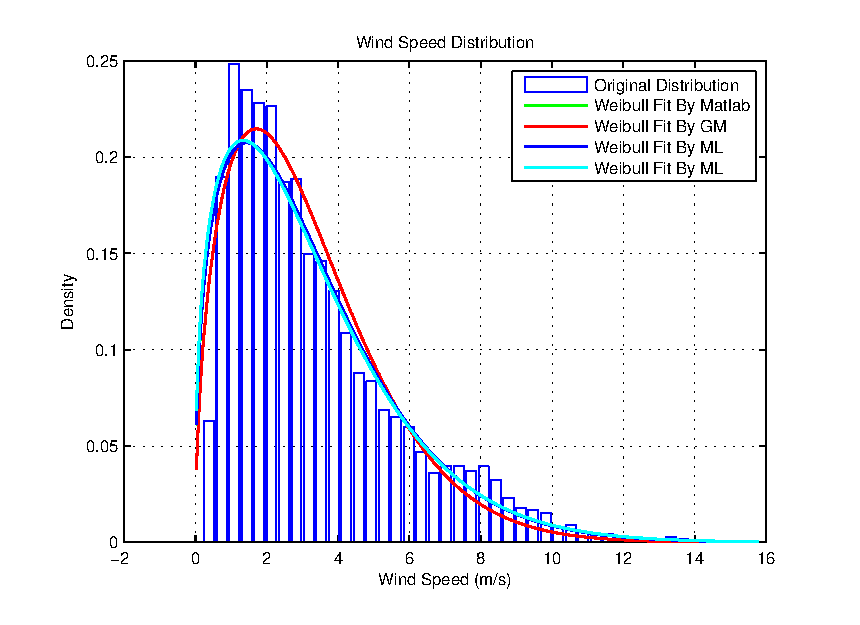
\includegraphics[width={12cm}]{fig/example.eps}
\caption{This is an example by using method 1}
\label{fig:example1}
\end{figure}



\section{Section 2.2}\label{sec:s22}

\subsection{Subsection 2.2.1}\label{subsec:s211}

Method 2: Use the XJTLU efigure command in Fig \ref{fig:example}

\efigure{This is an example by using method 2}{example}{12cm}

\chapter{chapter 3}\label{cpt:c3}

You can compile your tex file by Ctrl + Shift + L and compile the
citation file by Ctrl + Shift + B. After some times compile, you can use the
menu Tex - PDF - dvi2pdf to get the pdf file.

The official document will be published later.

\appendix
\chapter{Matlab Code}

\lstinputlisting[language=Matlab]{code/code.m}

\bibliographystyle{ieeebib}
\bibliography{reference}
\addcontentsline{toc}{chapter}{Reference}
\end{document}
